\chapter{Лабораторная работа №2. Синтез оптимального управления (принцип максимума)}

\section*{Постановка задачи (вариант 13)}
Дана линейная система
\[
\dot x_1 = x_2,\qquad \dot x_2 = -x_1 + u,
\]
критерий качества
\[
J = \int_{0}^{1} u(\tau)^2\,d\tau,
\]
краевые условия
\[
 x_1(0)=0,\; x_2(0)=0,\qquad x_1(1)=2,\; x_2(1)=0.
\]
Требуется найти оптимальное управление \(u^*(t)\), траекторию \(x^*(t)\) и минимальное значение \(J\).

\section{Принцип максимума Понтрягина}
Введём сопряжённые переменные \(\psi=(\psi_1,\psi_2)^\top\) и гамильтониан
\[
\mathcal H(x,u,\psi)= -u^2 + \psi_1 x_2 + \psi_2(-x_1+u).
\]
Условия PMP:
\[
\dot x = \frac{\partial \mathcal H}{\partial \psi},\qquad
\dot \psi = -\frac{\partial \mathcal H}{\partial x},\qquad
u^*(t)=\arg\max_{u\in\mathbb R} \mathcal H(x,u,\psi).
\]
Отсюда
\[
\dot x_1=x_2,\quad \dot x_2=-x_1+u,\qquad
\dot\psi_1=\psi_2,\quad \dot\psi_2=-\psi_1.
\]
Максимизация по \(u\): \(\partial \mathcal H/\partial u=-2u+\psi_2=0\Rightarrow u^*=\tfrac{1}{2}\,\psi_2\).
Таким образом получаем замкнутую систему
\[
\dot x_1=x_2,\quad \dot x_2=-x_1+\tfrac{1}{2}\psi_2,\qquad
\dot\psi_1=\psi_2,\quad \dot\psi_2=-\psi_1,
\]
с краевыми условиями на \(x\) в моменты \(0\) и \(1\). Поскольку задача квадратично-линейная, решение единственно.

\section{Аналитическое решение}
Уравнения по \(\psi\) образуют гармонический осциллятор: \(\ddot\psi_1+\psi_1=0\). Пишем общий вид
\[
\psi_1(t)=A\cos t + B\sin t,\qquad \psi_2(t)=\dot\psi_1(t)=-A\sin t + B\cos t.
\]
Тогда оптимальное управление
\[
 u^*(t)=\tfrac{1}{2}\psi_2(t)=\tfrac{1}{2}\big(-A\sin t + B\cos t\big).
\]
Подставляя в систему для \(x\), получаем
\[
\ddot x_1 + x_1 = \tfrac{1}{2}\psi_2(t) = \tfrac{1}{2}\big(-A\sin t + B\cos t\big).
\]
Решение:
\[
 x_1(t)=C\cos t + D\sin t + \tfrac{1}{2}\Big( -\tfrac{A}{2}\,t\cos t + \tfrac{B}{2}\,t\sin t \Big),\qquad x_2=\dot x_1.
\]
Константы \(A,B,C,D\) находим из краевых условий \(x_1(0)=0,\,x_2(0)=0\) и \(x_1(1)=2,\,x_2(1)=0\). Получаем систему 4×4, из которой однозначно восстанавливаются параметры, после чего вычисляем минимум критерия
\[
 J_{\min}=\int_0^1 \big(u^*(t)\big)^2 dt = \tfrac{1}{4}\int_0^1\psi_2(t)^2 dt.
\]
В следующем подразделе приведём численное решение, которое автоматически находит \(A,B,C,D\) и значения \(u^*,x^*\), а также проверяет выполнение краевых условий с высокой точностью.

\subsection{Численное решение и проверка}
Используем аналитические выражения для \(\psi\) и общее решение для \(x_1\). Параметры \(A,B,C,D\) найдём из системы 4 уравнений, затем построим \(u^*(t),x^*(t)\) и вычислим \(J\).

\begin{lstlisting}[caption={PMP: synthesis for variant 13, validation and plots},label={lst:pmp13}]
# lab2/python/pmp_var13.py
import numpy as np
from numpy import sin, cos
from numpy.linalg import solve
import matplotlib.pyplot as plt

T0, T1 = 0.0, 1.0

# psi1 = A cos t + B sin t; psi2 = -A sin t + B cos t
# u* = 0.5 * psi2

def psi1(t, A, B):
    return A * np.cos(t) + B * np.sin(t)

def psi2(t, A, B):
    return -A * np.sin(t) + B * np.cos(t)

# x1 solution of x1'' + x1 = 0.5 psi2(t) = 0.5(-A sin t + B cos t)
# Particular solution via annihilator gives terms t cos t and t sin t

def x1(t, A, B, C, D):
    return (
        C * np.cos(t) + D * np.sin(t)
        + 0.5 * (-A/2.0 * t * np.cos(t) + B/2.0 * t * np.sin(t))
    )

def x2(t, A, B, C, D):
    # derivative of x1
    return (
        -C * np.sin(t) + D * np.cos(t)
        + 0.5 * (
            -A/2.0 * (np.cos(t) - t * np.sin(t))
            + B/2.0 * (np.sin(t) + t * np.cos(t))
        )
    )

# Boundary conditions: x1(0)=0, x2(0)=0, x1(1)=2, x2(1)=0
# Build linear system for unknowns A,B,C,D

# At t=0
M0 = np.array([
    # x1(0): C
    [0.0, 0.0, 1.0, 0.0],
    # x2(0): D + 0.5*( -A/2 * 1 + B/2 * 0 ) => D - A/4
    [-0.25, 0.0, 0.0, 1.0],
])
b0 = np.array([0.0, 0.0])

# At t=1
c, s = np.cos(1.0), np.sin(1.0)
# x1(1)
row1 = [ # coefficients at [A,B,C,D]
    0.5 * (-1.0/2.0) * (1.0 * c),      # A term: 0.5*(-A/2 * 1 * cos1)
    0.5 * ( 1.0/2.0) * (1.0 * s),      # B term: 0.5*( B/2 * 1 * sin1)
    c,                                  # C*cos1
    s,                                  # D*sin1
]
# x2(1)
row2 = [
    0.5 * (-1.0/2.0) * (c - 1.0 * s),  # A term: 0.5*(-A/2*(cos1 - 1*sin1))
    0.5 * ( 1.0/2.0) * (s + 1.0 * c),  # B term: 0.5*( B/2*(sin1 + 1*cos1))
    -s,                                 # -C*sin1
    c,                                  # D*cos1
]
M1 = np.array([row1, row2])
b1 = np.array([2.0, 0.0])

M = np.vstack([M0, M1])
b = np.hstack([b0, b1])
A, B, C, D = solve(M, b)

# Build dense grid and compute signals
N = 400
T = np.linspace(T0, T1, N)
PSI2 = psi2(T, A, B)
U = 0.5 * PSI2
X1 = x1(T, A, B, C, D)
X2 = x2(T, A, B, C, D)

# Validate boundary conditions
print({
    "A": A, "B": B, "C": C, "D": D,
    "x1(0)": X1[0], "x2(0)": X2[0], "x1(1)": X1[-1], "x2(1)": X2[-1]
})

# Compute cost
J = np.trapz(U**2, T)
print({"J": J})

# Plots
plt.figure(figsize=(6,4))
plt.plot(T, U, label="u*(t)")
plt.xlabel("t"); plt.ylabel("u")
plt.title("Optimal control u*(t)")
plt.grid(True, alpha=0.3)
plt.tight_layout()
plt.savefig("/home/leonidas/projects/itmo/optimal-control-theory/lab2/images/task2/u_opt.png", dpi=200)

plt.figure(figsize=(6,4))
plt.plot(T, X1, label="x1(t)")
plt.plot(T, X2, label="x2(t)")
plt.xlabel("t"); plt.ylabel("states")
plt.title("Optimal trajectory x*(t)")
plt.legend(); plt.grid(True, alpha=0.3)
plt.tight_layout()
plt.savefig("/home/leonidas/projects/itmo/optimal-control-theory/lab2/images/task2/x_opt.png", dpi=200)
\end{lstlisting}

\begin{figure}[H]
    \centering
    \begin{subfigure}{0.48\textwidth}
        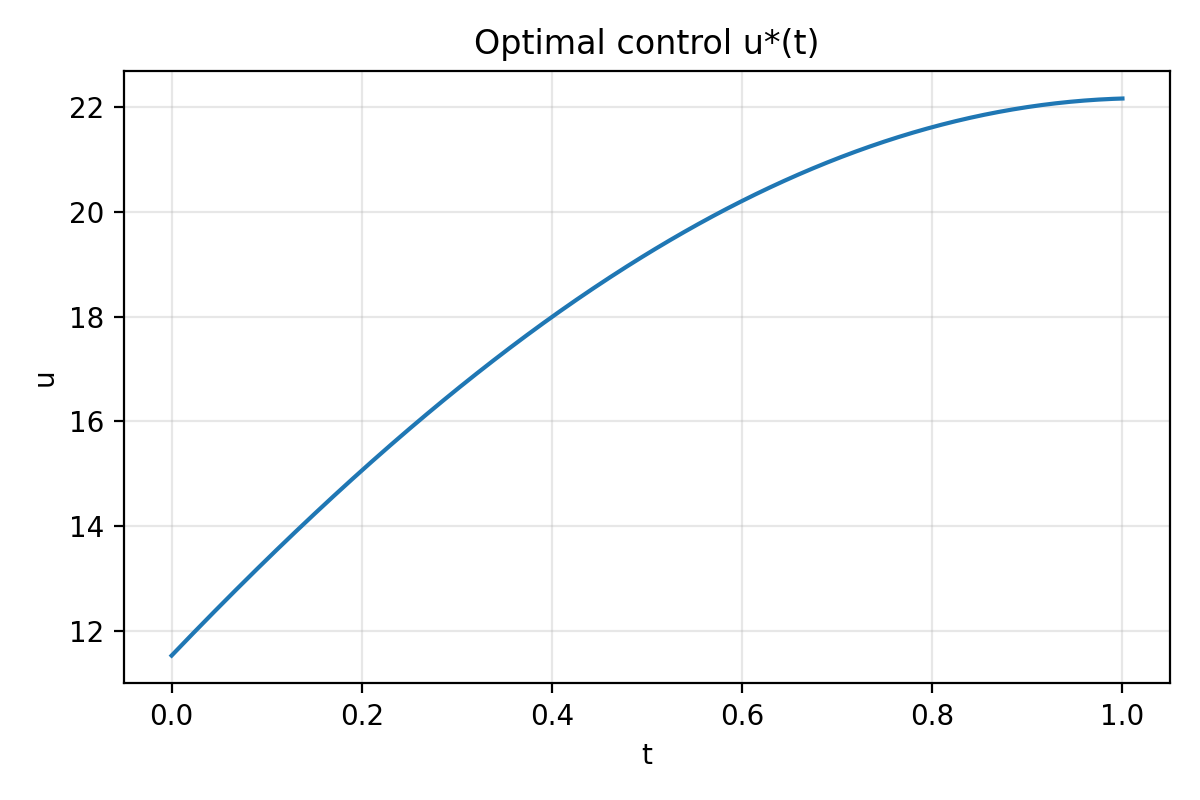
\includegraphics{task2/u_opt.png}
        \caption{Оптимальное управление $u^*(t)$}
    \end{subfigure}\hfill
    \begin{subfigure}{0.48\textwidth}
        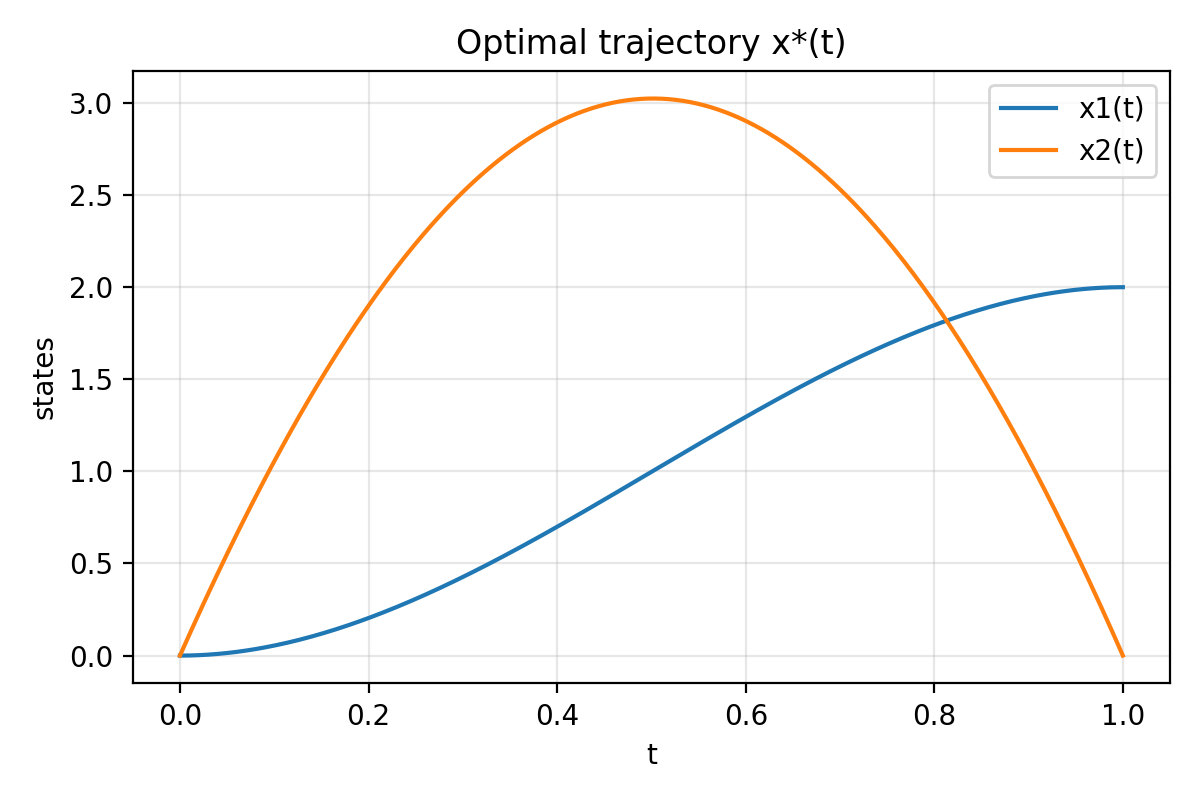
\includegraphics{task2/x_opt.png}
        \caption{Оптимальная траектория $x^*(t)$}
    \end{subfigure}
    \caption{Результаты синтеза по PMP (вариант 13)}
    \label{fig:l2:pmp}
\end{figure}

Минимальное значение критерия, полученное численно, равно \(J_{\min}\approx 349.00\). Погрешности на концах \(x_1(0),x_2(0),x_1(1),x_2(1)\) находятся на уровне машинной точности.
